\section{Theorie}
\label{sec:Theorie}

\subsection{Terminologie und Definitionen der Festkörperphysik}
\label{sec:terminologie}
Die effektive Masse $m*$ ist eine Definition für die Masse von Elektronen, um die 
Wechselwirkung mit benachbarten Teilchen in einem Gitter zu berücksichtigen. 
Es gibt keine Möglichkeit, Elektronen in einer Gitterstruktur zu bewegen, ohne 
effektive benachbarte Teilchen zu beeinflussen. Daher unterscheidet sich die 
Nettomenge, um die das Elektron beschleunigt wird (bei Kraftauswirkung) von 
dem tatsächlichen Literaturwert. Sie hängt direkt mit der zweiten Ableitung 
der Energie im Impulsraum zusammen. Dieses Konzept ist auch in dem Bändermodell 
wiederzufinden. Die sogenannte Bandstruktur  beschreibt die Zustände von Elektronen 
und Löchern eines kristallinenen Festkörpers im Impulsraum. Ein Beispiel befindet 
sich in \autoref{fig:1}. Es wird unterschieden zwischen den vollbesetzten 
Valenzbändern (am Nullpunkt) und den nächsthöheren Leitungsbändern. Für Metalle 
liegt die Fermi-Energie in mindestens einem dieser Bänder. Bei Halbleitern liegt 
sie dazwischen, in der Bandlücke. Da die effektive Masse abhängig von 
$\partial^2 \epsilon / \partial k^2$ ist, ist $m* < m$ bei starker Krümmung
und $m* > m$ bei leichter Krümmung.
\begin{figure}[H]
    \centering
        \centering
        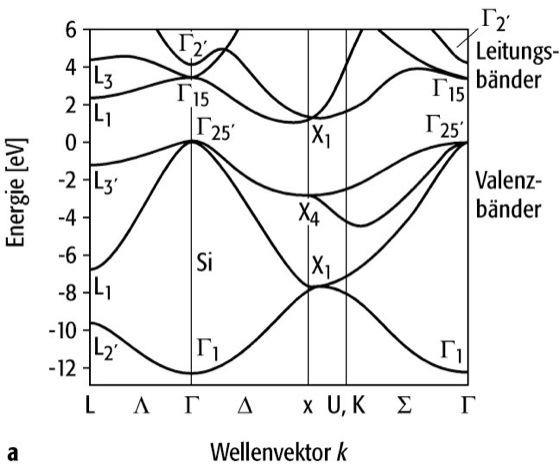
\includegraphics[width=0.5\textwidth]{Bilder/bandSi.jpg}
        \caption{Bandstruktur von Silizium. \cite{bandSi}}
    \hfill
    \label{fig:1}
\end{figure}
\noindent Ebenso wichtig ist die Dotierung, mit dessen Hilfe kann die Leitfähigkeit 
von Halbleitern erhöht werden, indem gezielt Atome mit Elektronenüberschuss 
oder Elektronenmangel eingebaut werden. Es wird unterschieden zwischen p- und 
n-Dotierungen. Bei der p-Dotierung wird ein Atom mit einer geringeren 
Valenzelektronenzahl hinzugefügt (Akzeptor) und bei der n-Dotierung ein Atom mit
einer Höheren (Donator). Die Energieniveaus von Donatoren befinden sich in der 
Bandstruktur demnach unterhalb des Leitungsbandes, es gibt bei thermischer
Erhitzungein ein Elektron ab. Ein Akzeptor liegt über dem Leitungsband, er nimmt 
ein Elektron auf, sobald thermische Energie hinzugefügt wird.

\subsection{Zirkulare Doppelbrechung}
Einige kristalline Festkörper verfügen über die Möglichkeit, die Polarisationsrichtung 
von Licht zu ändern. Das kann beispielsweise bei anisotropen Materialien der Fall 
sein, da diese unterschiedliche Brechungsindizes $n$ haben und Licht in ihnen 
dementsprechend unterschiedlich gebrochen werden kann. 
\vspace{0.5em}
\\
Linear polarisiertes Licht besteht aus links-und rechts zirkular polarisierten 
Wellen, welche phasenidentisch verlaufen. Diese Entartung kann aufgehoben werden,
indem die Phasengeschwindigkeiten verändert und damit die Phasen variiert werden. 
Wenn nun linear polarisiertes Lich auf einen doppelbrechenden Kristall trifft, 
findet dieser Effekt statt: der Lichtstrahl wird in zwei kollineare zirkular 
polarisierte Lichtstrahlen aufgeteilt (mit unterschiedlicher Phasengeschwindigkeit).
Sobald das Licht wieder austritt, vereinen sich die Komponenten erneut zu einem 
linear polarisierten Lichtstrahl. Dieser austretende Strahl hat jetzt eine 
Polarisationsebene, welche sich um einen Winkel $\theta$ zur eintretenden Ebene 
unterscheidet.
\begin{figure}[H]
    \centering
        \centering
        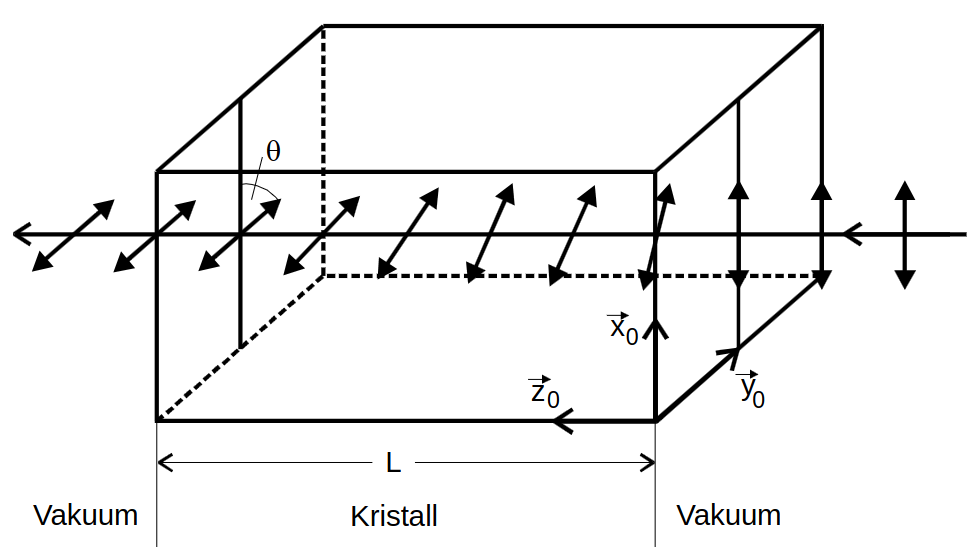
\includegraphics[width=0.5\textwidth]{Bilder/zBrechung.png}
        \caption{Veranschaulichung der Änderung der Polarisationsebene an einem Kristall. \cite{v46anhang}}
    \hfill
    \label{fig:2}
\end{figure}

\subsection{Faraday Effekt und die Bestimmung der effektiven Masse}
Bei dem Faraday Effekt handelt es sich um eine induzierte Doppelbrechung: er
beschreibt die Rotation einer Polarisationsebene einer linear polarisierten 
elektromagnetischen Welle, wenn ein Magnetfeld angelegt ist, welches parallel
zur Ausbreitungsrichtung der Welle liegt (siehe \autoref{fig:3}).
\vspace{0.5em}
\\
Zur Bestimmung der effektiven Masse mittels des Faraday-Effekts wird zunächst
der Kristall im feldfreien Zustand betrachtet. Aufgrund der Isotropie ist der
Suszeptibilitätstensor $\chi$ diagonal, wodurch die Polarisation $\vec{P}$ 
parallel zum elektrischen Feld $\vec{E}$ steht. Sobald $\vec{B} \neq 0$, erzwingt 
die Lorentzkraft Änderungen in den Bewegungen der Elektronen, es werden Dipole
induziert. Dadurch ist $\vec{P} \nparallel \vec{E}$ und $\chi$ verliert seine 
Diagonalgestalt. Das Medium ist in diesem Fall anisotrop geworden. Da sich die 
Wellenzahlen $k_L$ und $k_R$ unterscheiden, weil die sich die links- und 
rechtszirkulare nicht mehr so überlagern wie vorher, unterscheiden sich auch 
Wellengeschwindigkeiten: es kommt zur zirkularen Doppelbrechung und infolgedessen 
zur Rotation der Polarisationsachse.
\\
Aus der Bewegungsgleichung eines gebundenen Elektrons im elektrischen Feld der
Lichtwelle und dem äußeren Magnetfeld ergibt sich nach Elimination der
Polarisationsvariablen einen Ausdruck für den Faraday-Rotationswinkel $\theta$:
\begin{equation}
    \label{eqn:1}
    \theta \approx \frac{e_0^3}{2 \epsilon_0 c m^2} \frac{\omega}{(\omega_0^2 -
     \omega)^2} \frac{N B L}{n}.
\end{equation}
Dabei wurde angenommen, dass die Resonanzfrequenz $\omega_0$ sowie Messfrequenzen 
bei Halbleitern im Infrarotbereich liegen, sodass $(\omega_0^2 -\omega)^2 >> \omega^2 \omega_c^2$
(mit $\omega_c$, der Zyklotonfrequenz). Für eine zusätzliche Vernachlässigung der 
Bindungskräfte folgt
\begin{equation}
    \label{eqn:2}
    \theta = \frac{e_0^3}{8 \pi \epsilon_0 c^3} \frac{1}{(m*)^2} \frac{\lambda^2 N B}{n}.
\end{equation}
Diese Näherung ist sinnvoll, da bei der n-dotierten Probe die Ladungsträger 
quasifrei sind. Die rücktreibende Kraft kann vernachlässigt werden, da die 
Elektronen nicht an einzelne Atomrümpfe gebunden sind. Mathematisch wird das 
durch den Fall $\omega_0 \rightarrow 0$ realisiert. Für die effektive Masse 
wird umgestellt. Die gesuchte Größe kann mittels 
\begin{equation}
    \label{eqn:3}
    m* = \sqrt{\frac{e_0^3}{8 \pi \epsilon_0 c^3} \frac{1}{\theta} \frac{\lambda^2 N B}{n}}
\end{equation}
berechnet werden. \cite{v46anhang}
\begin{figure}[H]
    \centering
        \centering
        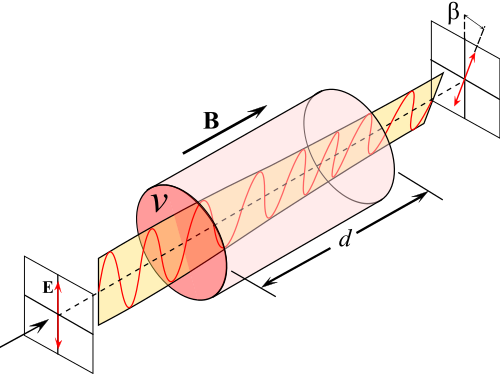
\includegraphics[width=0.5\textwidth]{Bilder/FaradayEffekt.png}
        \caption{Schematische Funktionsweise des Faraday'schen Effekts. \cite{faraday_img}}
    \hfill
    \label{fig:3}
\end{figure}


\subsection{Fehlerrechnung}
Die gemessenen Werte unterliegen Messunsicherheiten und werden demnach im
Folgenden nicht als fehlerfrei angesehen. Die Fehler entstehen bei der
Bildung der Mittelwerte durch den Fehler des Mittelwerts und bei der
Regressionsrechnung sowie der Fehlerforpflanzung durch Python.
Der Mittelwert ist definiert durch
\begin{equation}
    \overline{x} = \frac{1}{N} \sum\limits_{i=1}^N x_i.
\end{equation}
\noindent Der Fehler des Mittelwerts ist somit gegeben durch 
\begin{equation}
    \begin{aligned}
        \increment \overline{x} &= \sqrt{\overline{x^2\kern-0.1em} - \overline{x}^2} \\
                            &= \frac{\sqrt{\frac{1}{N-1} \sum\limits_{i=1}^N (x_i - \overline{x})^2}}{\sqrt{N}}.
    \end{aligned}
\end{equation}

\noindent Um Fehler einzubeziehen, wird die Gauß'sche Fehlerfortpflanzung verwendet:
\begin{equation}
    \label{eqn:9}
    \increment f = \sqrt{\left(\frac{\partial f}{\partial x}\right)^2 \cdot \left(\increment x\right)^2 + \left(\frac{\partial f}{\partial y}\right)^2 \cdot \left(\increment y\right)^2 + .... + \left(\frac{\partial f}{\partial z}\right)^2 \cdot \left(\increment z\right)^2}
\end{equation}